% =====================================================================
% ARTIGO FINAL — Reescrita completa (George, ABNT autor-data)
% Detecção e Mitigação Inteligente de Anomalias em SDN com LLMs Open
% Source: correlação Projeto de Pesquisa (goal.pdf) x Sistema NOC Lite.
% Codificação: UTF-8 / pdflatex (TinyTeX).
% Citacao ABNT autor-data via abntex2cite (estilo alf).
% Compilação: pdflatex -> bibtex -> pdflatex -> pdflatex.
% Bibliografia unica: referencias_autor_data.bib (versao curada).
% Sem tags editoriais; sem bullet points nas secoes narrativas.
% =====================================================================
\documentclass[12pt,a4paper]{article}

\usepackage[utf8]{inputenc}
\usepackage[T1]{fontenc}
\usepackage{indentfirst}

% --- Citacao ABNT autor-data (NBR 10520) via abntex2cite ---
\usepackage[alf]{abntex2cite}

% --- Utilitarios ---
\usepackage{graphicx}
\usepackage{hyperref}
\usepackage{float}
\usepackage{longtable}
\usepackage{booktabs}
\usepackage{amsmath}
\usepackage{caption}

% --- Hiperlinks em preto (evita caixas coloridas na impressão) ---
\hypersetup{colorlinks=true, linkcolor=black, citecolor=black,
            urlcolor=black, pdfborder={0 0 0}}

\graphicspath{{../figures/}{figuras/}}

\title{\textbf{Detecção e Mitigação Inteligente de Anomalias em Redes
Definidas por Software com Grandes Modelos de Linguagem Open Source:
correlação entre o Projeto de Pesquisa e o Sistema Implementado (NOC Lite)}}

\author{Estudo de correlação elaborado a partir do Projeto de Pesquisa
de Rodrigues (2026, Edital n\textsuperscript{o} 26/2026) e do
sistema \textit{NOC Lite} implementado \\[2mm]
\textit{Artigo técnico-científico — revisão integrativa e análise
arquitetural}}

\date{Julho de 2026}

\begin{document}
\maketitle

% =====================================================================
\begin{abstract}
A detecção e a mitigação inteligente de anomalias em redes definidas por
software têm sido reconfiguradas pela adoção de grandes modelos de
linguagem \textit{open source}, ajustados por técnicas de fine-tuning
eficiente em parâmetros, como LoRA e QLoRA, em substituição a modelos
fechados e a abordagens puramente reativas. O presente trabalho correlaciona
o projeto de pesquisa que propõe esse paradigma -- voltado a anomalias de
desempenho em SDN, com reconfiguração de topologia virtual em ciclo fechado
-- com o sistema efetivamente implementado, denominado \textit{NOC Lite}.
A partir de uma revisão da literatura estruturada em seis eixos (SDN/NFV,
anomalias por aprendizado de máquina tradicional, LLMs \textit{open source}
para NetOps, PEFT/LoRA/QLoRA, inteligência artificial explicável e
geração de cenários anômalos com datasets públicos), descreve-se a
arquitetura e o pipeline de classificação do sistema construído, composto
por três classificadores (heurístico, árvore de decisão e IA generativa
via Google Gemini). Em seguida, apresenta-se o mapeamento
artigo$\times$sistema e a taxonomia de gaps estruturais, destacando-se a
ausência de SDN, o uso de modelo fechado em vez de LLM \textit{open
source}, a inexistência de ajuste fino LoRA/QLoRA, a falta de mitigação em
ciclo fechado e a dependência exclusiva de dados sintéticos. Discutem-se as
convergências preservadas (baselines, tokenização, justificativa textual,
métricas de latência) e propõem-se diretrizes de arquitetura para o
alinhamento futuro, incluindo um ciclo fechado com LLM local, LoRA e módulo
de mitigação. Conclui-se que o \textit{NOC Lite} realiza parcela da
intenção do projeto, mas exige evolução arquitetural substantiva nos eixos
centrais para aproximar-se da proposta norteadora.
\end{abstract}

\noindent\textbf{Palavras-chave:} Redes Definidas por Software; Anomalias de
Rede; Grandes Modelos de Linguagem; PEFT/LoRA; Inteligência Artificial
Explicável.

\vspace{6pt}
\hrule
\vspace{10pt}

% =====================================================================
\section{Introdução}
\label{sec:intro}

Redes de computadores modernas operam sob demandas cada vez mais rigorosas
de desempenho, confiabilidade e segurança, em um cenário marcado pela
heterogeneidade de aplicações e pela complexidade crescente da
infraestrutura distribuída. Nesse contexto, a identificação e a
classificação de fenômenos anômalos -- congestionamento transiente, falhas
de enlace, degradação de desempenho -- tornam-se atividades fundamentais
para a operação eficiente de sistemas computacionais, uma vez que a
degradação silenciosa de métricas de rede frequentemente antecede falhas
operacionais de maior impacto \cite{rRODRIGUES}. Tradicionalmente, a
análise de anomalias depende de intervenção manual e de conhecimento
especializado, o que a torna propensa a erros e com baixa agilidade de
adaptação em tempo real \cite{rA39}. Modelos baseados em assinaturas ou
regras pré-definidas são frequentemente reativos e possuem capacidade
limitada para detectar ameaças desconhecidas ou comportamentos de
desvio sutil, especialmente quando a fronteira entre operação normal e
anômala é difusa \cite{rA512}.

Nos últimos anos, grandes modelos de linguagem demonstraram capacidades de
interpretação, raciocínio contextual e generalização a partir de descrições
textuais e dados estruturados \cite{rA31}. Diferentemente de classificadores
tradicionais, tais modelos conseguem combinar múltiplas informações, lidar
com incertezas e produzir não apenas uma decisão, mas também uma
justificativa textual compatível com a análise humana \cite{rA321}. O
paradigma das redes definidas por software, ao separar o plano de controle do
plano de dados, fornece a agilidade necessária para que agentes de
inteligência artificial percebam o estado da rede e executem ações de
otimização ou segurança de forma autônoma \cite{rA19}. Essa convergência --
controle programável por software e raciocínio generativo -- constitui a
motivação central do projeto de pesquisa norteador deste estudo.

O projeto de pesquisa propõe desenvolver um sistema autônomo baseado em
LLMs \textit{open source} (ex.: Llama, Falcon) e em ajuste fino eficiente de
parâmetros (PEFT), notadamente LoRA/QLoRA, para detectar anomalias de
performance em SDN e mitigá-las via reconfiguração proativa de topologia
virtual (VNT) e roteamento, em ciclo fechado \cite{rRODRIGUES}. O projeto
exige, ainda, a utilização de datasets públicos consagrados para validação
cruzada, a conversão de atributos numéricos em representações textuais e a
entrega de justificativas textuais interpretáveis. Contudo, o sistema
implementado -- o \textit{NOC Lite} -- monitora \textit{hosts} genéricos
(endereços IP/DNS) por sondas ICMP/TCP/HTTP/DNS/SNMP, emprega o modelo
fechado Google Gemini como classificador generativo e não realiza mitigação
nem reconfiguração de rede. Há, portanto, uma distância estrutural entre a
proposta do projeto e o sistema construído.

Essa distância motiva a presente análise, que se justifica pela escassez de
estudos que confrontem, com evidência de código, uma proposta de pesquisa de
LLMs \textit{open source} para SDN e sua implementação concreta. Os
objetivos deste trabalho são: expor o referencial teórico das seis áreas de
conhecimento envolvidas; descrever o sistema implementado e seu pipeline de
classificação; apresentar o mapeamento projeto$\times$sistema e a taxonomia
de gaps; discutir convergências, limitações e ameaças à validade; e propor
diretrizes de arquitetura para o alinhamento futuro. A contribuição deste
artigo é a caracterização sistemática e fundamentada em evidência de código
da lacuna entre uma proposta de pesquisa de LLMs \textit{open source} para
SDN e sua implementação, servindo tanto como diagnóstico quanto como
roteiro de evolução.

% =====================================================================
\section{Referencial Teórico e Revisão da Literatura}
\label{sec:referencial}

A fundamentação deste trabalho articula seis eixos de conhecimento,
sintetizados a partir de revisão de literatura estruturada, com as
referências citadas validadas nos relatórios de estado da arte do próprio
projeto. A seleção do corpus seguiu um procedimento de revisão integrativa
\cite{rA28,rA212}, partindo de seis áreas de conhecimento mapeadas a partir
do projeto de pesquisa norteador \cite{rRODRIGUES} e de relatórios de
análise de código do sistema \textit{NOC Lite}: (1) SDN/NFV; (2) detecção e
classificação de anomalias por aprendizado de máquina tradicional; (3) LLMs
\textit{open source} e modelos de linguagem para NetOps; (4) fine-tuning
eficiente de LLMs (PEFT/LoRA/QLoRA); (5) inteligência artificial explicável
(XAI); e (6) geração de cenários anômalos e datasets públicos. Como
critérios de inclusão, admitiram-se obras primárias (artigos, preprints e
relatórios técnicos) diretamente relacionadas a um dos seis eixos e com
relevância para a análise arquitetural realizada; excluíram-se trabalhos
fora do escopo de detecção/mitigação de anomalias em redes e fontes sem
validação verificável. O corpus final compreende as fontes efetivamente
citadas, distribuídas pelos seis eixos, consolidadas em uma única lista de
referências ordenada alfabeticamente conforme a ABNT NBR 6023.

\subsection{Redes Definidas por Software e Virtualização de Funções de Rede}
\label{sec:sdn}

O paradigma SDN desacopla o plano de controle do plano de dados por meio de
um protocolo southbound padronizado (OpenFlow) \cite{rA11} e de
controladores programáveis (NOX \cite{rA12}, POX, Ryu \cite{rA116},
OpenDaylight \cite{rA114}, ONOS \cite{rA115}). Essa centralização lógica
cria uma única fonte de verdade e uma superfície de programação que,
simultaneamente, facilita a automação e introduz novas superfícies de ataque
no plano de controle \cite{rA122,rA123,rA124}. A emulação (Mininet
\cite{rA14}, Open vSwitch \cite{rA15}) viabiliza a geração controlada de
cenários anômalos \cite{rA19}. Surveys definitivos consolidam a taxonomia e
os desafios de segurança da SDN \cite{rA19,rA110}, fornecendo o vocabulário
exato -- tabelas de fluxo, contadores, regras -- que um agente de
inteligência artificial deve compreender para atuar sobre a rede.

Complementarmente, a Virtualização de Funções de Rede (NFV), institucionalizada
pelos white papers e pelo framework arquitetural da ETSI \cite{rA127,rA128,rA129},
e revisitada por Mijumbi et al. \cite{rA130,rA131} e Laghrissi \& Taleb
\cite{rA132}, estende o paradigma ao ciclo de vida de funções virtualizadas e
sua orquestração (MANO). Sobre esse alicerce, o Intent-Based Networking (IBN)
emerge como a camada de gestão que traduz objetivos de alto nível em
configurações concretas e as garante por meio de laços fechados
\cite{rA133}. Trabalhos como Morales et al. \cite{rA134} e a survey de
Panayiotou et al. \cite{rA135} antecipam a reconfiguração proativa da
topologia virtual orientada a dados e a aprendizado de máquina. A detecção
de anomalias em SDN transita, assim, de métodos clássicos de ML
\cite{rA126} para a integração de LLMs \textit{open source} ajustados por
LoRA/QLoRA, exatamente o movimento defendido pelo projeto norteador.

\subsection{Detecção e Classificação de Anomalias por Métodos Tradicionais}
\label{sec:ml}

A literatura consolida que métodos estatísticos (cartas EWMA \cite{rA22},
Holt-Winters \cite{rA21}, ARIMA/SARIMA \cite{rA25,rA27}) e classificadores de
ML clássico (SVM \cite{rA213}, Random Forest \cite{rA210}, árvores de
decisão \cite{rA217}, redes rasas \cite{rA231}) formam o arcabouço de
baselines sobre o qual a detecção moderna é avaliada. Surveys consagrados
\cite{rA28,rA29,rA210,rA212} reforçam que heurísticas de limiar e modelos
estatísticos são insubstituíveis como referência de comparação por serem
interpretáveis e leves, propriedade particularmente valiosa para operadores
de NOC. Para os tipos de anomalia do sistema, há corpus dedicado e real: o
DDoS é coberto por baselines de árvore/Random Forest \cite{rA222,rA224,rA225};
a varredura de portas possui precedentes heurísticos e de ML
\cite{rA227,rA229}; a exfiltração é abordada sobre metadados de fluxo
\cite{rA226}; e o congestionamento ou a falha de enlace encontra raiz em
detecção estatística de séries temporais \cite{rA21,rA232,rA21}. Tais
baselines não são meros artefatos históricos: constituem o termômetro
obrigatório contra o qual qualquer abordagem nova, incluindo LLMs, deve ser
medida em termos de acurácia, interpretabilidade e custo operacional.

\subsection{LLMs Open Source e Modelos de Linguagem para NetOps}
\label{sec:llm}

Surveys dedicados mapeiam a aplicação de LLMs à operação e gestão de redes
(NO\&M/NetOps) \cite{rA31,rA32,rA33,rA34,rA35,rA36,rA37}, estabelecendo o
arcabouço conceitual -- percepção, raciocínio, ação -- sobre o qual se
inscreve a classificação generativa de anomalias. O ecossistema de modelos
\textit{open source} -- LLaMA/Llama 2 \cite{rA310,rA311}, Mistral 7B
\cite{rA312}, Falcon \cite{rA313}, Qwen/Qwen2.5 \cite{rA314,rA315}, BLOOM
\cite{rA316} e, sobretudo, Gemma \cite{rA317} (derivado da tecnologia
Gemini) -- oferece pesos e licenças que tornam viável a substituição de
modelos fechados por alternativas locais e ajustáveis \cite{rA41}. A
arquitetura Transformer \cite{rA319}, o alinhamento por RLHF \cite{rA320} e o
Chain-of-Thought (CoT) \cite{rA321} fundamentam, respectivamente, a
capacidade de raciocínio, de seguir instruções e de produzir justificativa
textual. Aplicações concretas incluem detecção de anomalias em SDN
\cite{rA325,rA327}, IBN orientado a LLM \cite{rA324,rA332,rA333} e agentes de
rede autônomos \cite{rA338,rA334,rA335,rA336,rA337}, demonstrando que o
paradigma já ultrapassou a fase puramente conceitual.

\subsection{Fine-Tuning Eficiente de LLMs (PEFT): LoRA, QLoRA}
\label{sec:peft}

O ajuste fino eficiente (PEFT) -- liderado por LoRA \cite{rA41} e estendido
por QLoRA \cite{rA42}, AdaLoRA \cite{rA43} e DoRA \cite{rA44} -- é a via
consagrada para adaptar LLMs \textit{open source} a domínios específicos com
orçamento de hardware modesto, reduzindo em ordens de magnitude os parâmetros
treináveis sem overhead de inferência \cite{rA45,rA49,rA415}. Frameworks como
LLM-Adapters \cite{rA411} e LLaMA-Adapter \cite{rA412} demonstram que LLMs
7B ajustados por PEFT igualam ou superam modelos 175B em zero-shot. No
domínio de tráfego de rede, NetGPT \cite{rA425}, TrafficGPT \cite{rA426} e
TrafficLLM \cite{rA427} mostram que LLMs podem ser ajustados, com tokenização
de domínio, para entender e classificar tráfego. A base few-shot/zero-shot
(Brown \cite{rA422}, Wei \cite{rA321}, Achiam \cite{rA424}) legitima o uso de
LLMs sem ajuste de pesos, mas a literatura documenta que o PEFT tipicamente
supera o in-context learning em custo e acurácia \cite{rA49}, o que justifica
a exigência de LoRA/QLoRA no projeto norteador.

\subsection{Inteligência Artificial Explicável (XAI)}
\label{sec:xai}

A XAI é requisito fundamental para a adoção confiável de detectores em
domínios de alta responsabilidade \cite{rA52,rA531,rA517}. Em NLP, o survey
de Danilevsky et al. \cite{rA51} sistematiza como modelos de linguagem
produzem explicações; Ribeiro et al. \cite{rA53} (LIME) e Lundberg \& Lee
\cite{rA54} (SHAP) oferecem atribuição local. O protótipo HuntGPT
\cite{rA511} integra um detector de anomalias por ML a um LLM que entrega
justificativas textuais, referência explícita do projeto. Estudos recentes
exploram LLMs para detecção de intrusão explicável \cite{rA520,rA521} e
explicabilidade em SDN \cite{rA522}. A calibração e a confiança das
justificativas são temas ativos \cite{rA531,rA532,rA533,rA534}, pois
explicações de LLM podem ser plausíveis e incorretas, exigindo verificação
cruzada com atribuição numérica de features.

\subsection{Geração de Cenários Anômalos e Datasets Públicos}
\label{sec:datasets}

A literatura estabelece UNSW-NB15 \cite{rA61,rA62} e CSE-CIC-IDS2018
\cite{rA63,rA64} como benchmarks modernos, superando os obsoletos
KDD99/NSL-KDD \cite{rA65,rA66}. A geração dessas bases segue perfis
comportamentais e emulação (Mininet, GNS3, PNETLab) \cite{rA69,rA629}.
Datasets SDN específicos (InSDN \cite{rA610}, SNT, DDoS2019) e técnicas de
data augmentation (GAN/VAE/SMOTE) endereçam o desbalanceamento de classes
\cite{rA614,rA615,rA623}. A conversão de atributos numéricos em
representações textuais -- formalizada por AnoLLM \cite{rA616} e revisada em
surveys de LLMs em dados tabulares \cite{rA617,rA618} -- abre caminho para
detectores baseados em LLMs, eixo conectado diretamente à inferência do
sistema analisado \cite{rA630}. A ausência de validação cruzada contra tais
bases é, precisamente, um dos pontos de tensão entre o projeto e o sistema
implementado.

% =====================================================================
\section{O Sistema Implementado: NOC Lite}
\label{sec:sistema}

O \textit{NOC Lite} é um sistema de monitoramento de disponibilidade e
performance de \textit{hosts} genéricos, estruturado como um monolito modular
em FastAPI com persistência em SQLite e um front-end estático. A arquitetura
de contêineres cobre o front-end (HTML/JS), a API backend
(FastAPI/Uvicorn), o motor de monitoramento (\texttt{asyncio}), o
classificador de anomalias, o simulador, o notificador (Telegram) e o banco
de dados SQLite. Ponto crítico de arquitetura: o classificador de anomalias
\textbf{não participa do laço de monitoramento} -- é acionado sob demanda via
\texttt{GET /api/anomalies/classify}, jamais pelo \textit{MonitorEngine},
operando como ferramenta de diagnóstico e não como sensor integrado ao
pipeline de detecção.

\begin{figure}[H]
  \centering
  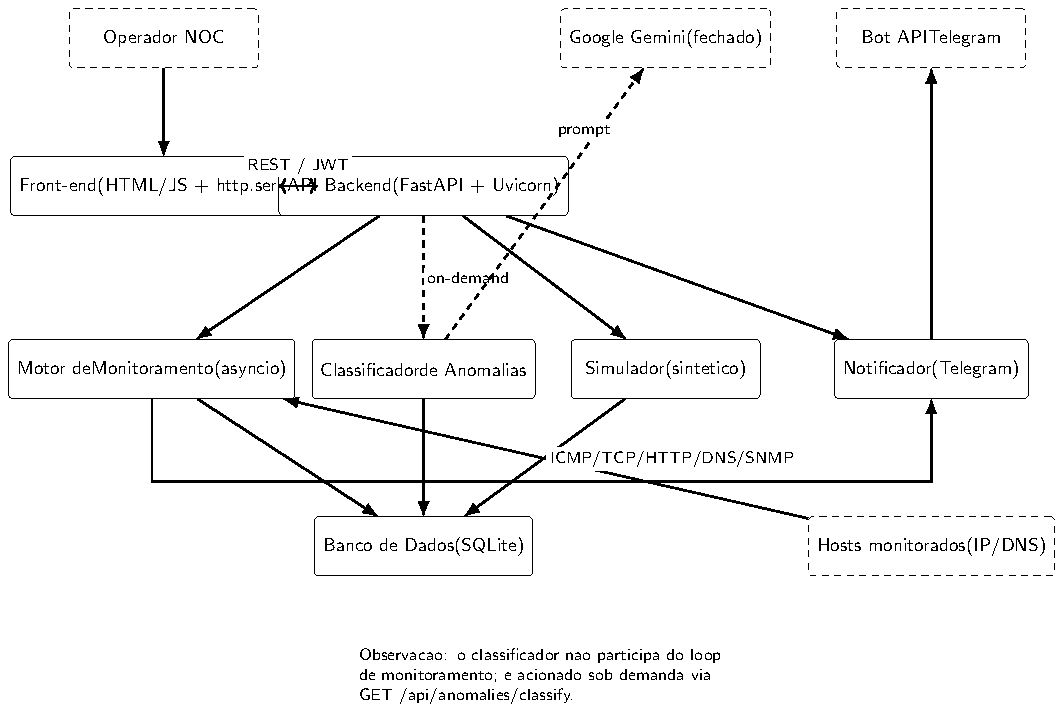
\includegraphics[width=0.85\textwidth]{fig_arquitetura_sistema}
  \caption{Arquitetura de contêineres do NOC Lite (C4, nível contêiner).
  Fonte: elaborada a partir de \texttt{arquitetura\_sistema.md} (Dan).}
  \label{fig:arq}
\end{figure}

\subsection{Pipeline de Classificação}
\label{sec:pipeline}

O subsistema de classificação expõe três estratégias sobre um conjunto
fechado de seis classes -- \texttt{NORMAL}, \texttt{DDOS\_ATTACK},
\texttt{PORT\_SCAN}, \texttt{HOST\_DOWN}, \texttt{DATA\_EXFILTRATION} e
\texttt{NETWORK\_CONGESTION} -- conforme o fluxo da Figura~\ref{fig:pipe}. A
primeira estratégia, o classificador heurístico (\texttt{classify\_heuristic}),
aplica regras de limiar estático sobre latência, CPU, memória e taxas de
sucesso de sondas; exemplos típicos são \texttt{network\_in\_bps > 50\,Mb/s}
e \texttt{cpu\_usage > 75} que levam a \texttt{DDOS\_ATTACK}, e
\texttt{ping\_latency > 120\,ms} que conduz a \texttt{NETWORK\_CONGESTION},
produzindo confiança fixa e explicação textual. A segunda, o classificador de
aprendizado de máquina (\texttt{classify\_ml}), utiliza um
\texttt{DecisionTreeClassifier(max\_depth=5)} do scikit-learn treinado
\textbf{exclusivamente com dados sintéticos} (1.200 amostras, 200 por
classe), sem PEFT e sem LLM, comportando-se, na prática, como uma
"árvore-cópia" da heurística. A terceira, a IA generativa
(\texttt{classify\_generative\_ai}), monta um prompt estruturado com o
snapshot tokenizado e o envia ao modelo fechado \texttt{gemini-1.5-flash},
retornando JSON com \texttt{classification}, \texttt{confidence} e
\texttt{explanation}, com fallback para a heurística em caso de falha.

\begin{figure}[H]
  \centering
  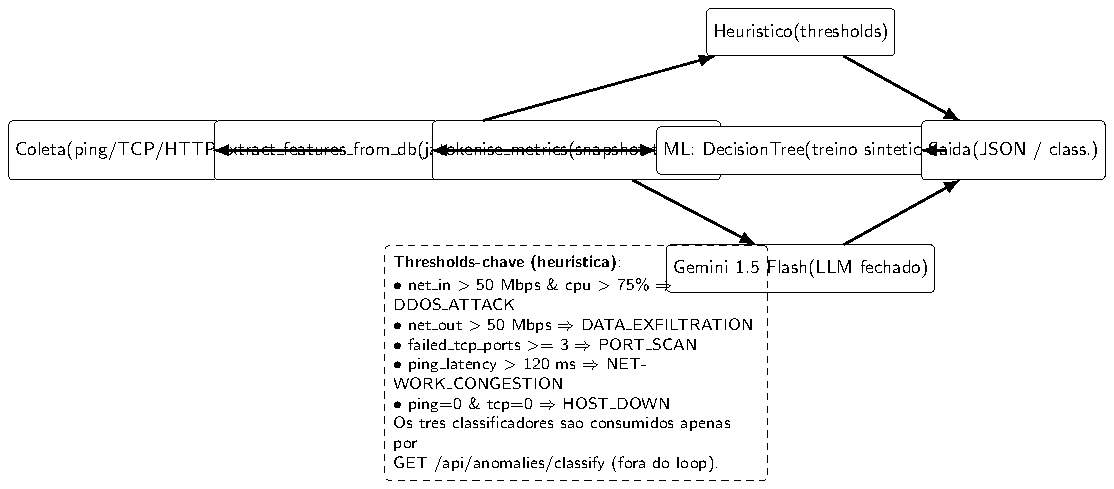
\includegraphics[width=0.78\textwidth]{fig_pipeline_classificacao}
  \caption{Pipeline de classificação de anomalias do NOC Lite: extração de
  features (janela de 5~min), três classificadores paralelos e tokenização
  para o LLM. Fonte: \texttt{notas\_coder.md} (John).}
  \label{fig:pipe}
\end{figure}

A função \texttt{tokenise\_metrics} converte o vetor numérico de dez
features em texto estruturado (ex.: \texttt{PingSuccessRate: 0.95 |
AvgPingLatency: 12.3 ms | CPUUsage: 34.1\%}), espelhando a recomendação do
projeto de converter atributos numéricos em representações textuais
\cite{rA616,rA431,rA432}. Esse texto é a ponte que permite ao LLM "ler" os
limiares de rede em linguagem natural, materializando o eixo de
serialização tabular$\rightarrow$texto discutido na fundamentação.

\subsection{Simulador}
\label{sec:sim}

O \texttt{anomaly\_simulator.py} gera cenários anômalos sintéticos
(\texttt{generate\_simulated\_metrics}) para as seis classes via
\texttt{random.uniform}, e injeta esses vetores diretamente no banco
(\texttt{run\_simulated\_check\_cycle}), podendo popular histórico
retroativo. O agendamento em tempo real usa estado em memória. Trata-se de
dados 100\% sintéticos, sem dependência de datasets públicos, o que confere
privacidade e reprodutibilidade, mas inviabiliza a comparação com o estado da
arte -- tensionando diretamente o requisito de validação cruzada do projeto.

% =====================================================================
\section{Mapeamento Projeto $\times$ Sistema e Gaps (Resultados)}
\label{sec:mapeamento}

A Tabela~\ref{tab:mapa} sintetiza a correspondência entre os
objetivos/componentes do projeto norteador \cite{rRODRIGUES} e o que o NOC
Lite efetivamente entrega, com o respectivo status de alinhamento. A
Figura~\ref{fig:mapa} ilustra essa relação de forma visual, evidenciando que
as convergências concentram-se nas margens do sistema (baselines,
tokenização, justificativa, métricas), ao passo que os eixos centrais da
proposta (SDN, LLM aberto, LoRA, mitigação, datasets) permanecem fora do
alcance implementado.

\begin{longtable}{cp{5.4cm}p{5.0cm}c}
\caption{Mapeamento Projeto de Pesquisa $\times$ NOC Lite.}
\label{tab:mapa}\\
\toprule
\textbf{\#} & \textbf{Objetivo/Componente do Projeto} & \textbf{Entrega do NOC Lite} & \textbf{Status} \\
\midrule
\endfirsthead
\toprule
\textbf{\#} & \textbf{Objetivo/Componente do Projeto} & \textbf{Entrega do NOC Lite} & \textbf{Status} \\
\midrule
\endhead
1 & LLM \textit{open source} (Llama/Falcon) com fine-tuning & Gemini 1.5 Flash (fechado); Árvore de Decisão & Divergente \\
2 & Fine-tuning PEFT (LoRA/QLoRA) & Inexistente; ML é árvore treinada do zero & Ausente \\
3 & Ambiente SDN virtualizado (Mininet/OVS) & Hosts IP genéricos; sondas ICMP/TCP/HTTP/DNS/SNMP & Ausente \\
4 & Mitigação via reconfiguração VNT/roteamento (ciclo fechado) & Apenas detecção + alerta Telegram; sem ação corretiva & Ausente \\
5 & Anomalias de performance (congestionamento, falha de enlace) & Mistura anomalias de segurança/operacionais com congest. genérico & Parcial \\
6 & Datasets públicos (UNSW-NB15, CIC-IDS2018, Synthetic SDN) & Dados 100\% sintéticos (random.uniform) & Divergente \\
7 & Baselines de comparação (heurística / ML) & Heurística + DecisionTree & Convergente \\
8 & Tokenização de métricas em texto estruturado & \texttt{tokenise\_metrics} & Convergente \\
9 & Justificativa textual (XAI) & \texttt{explanation} (com modelo fechado) & Convergente \\
10 & Avaliação de tempo de resposta por classificador & \texttt{latency\_ms} medido por classificador & Convergente \\
11 & Métricas resumidas (throughput, latência, jitter, perda) & SLA/jitter/tendência/health-score + SNMP & Convergente \\
12 & Ciclo fechado coleta$\rightarrow$classificação$\rightarrow$mitigação & Loop aberto: coleta$\rightarrow$severidade$\rightarrow$alerta & Aberto \\
\bottomrule
\end{longtable}

\begin{figure}[H]
  \centering
  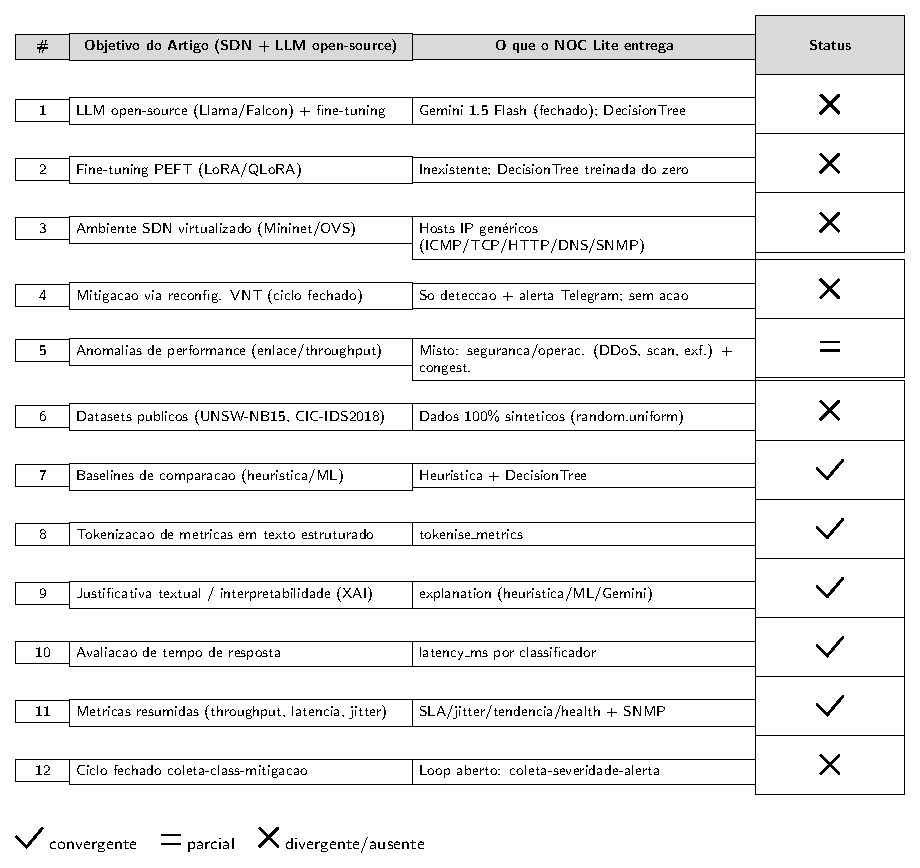
\includegraphics[width=0.85\textwidth]{fig_mapeamento_artigo_sistema}
  \caption{Mapeamento visual entre os objetivos do artigo norteador e o
  sistema NOC Lite. Fonte: elaborada por Chris.}
  \label{fig:mapa}
\end{figure}

\subsection{Taxonomia de Gaps}
\label{sec:gaps}

A análise arquitetural identifica sete gaps, sendo seis de severidade
crítica ou maior, conforme a Figura~\ref{fig:gaps}. Cada gap é sustentado
por evidência de código, conforme a Tabela~\ref{tab:gaps}.

\begin{longtable}{cp{4.0cm}p{8.0cm}c}
\caption{Taxonomia de gaps (NOC Lite $\times$ Projeto).}
\label{tab:gaps}\\
\toprule
\textbf{ID} & \textbf{Gap} & \textbf{Evidência no código / Descrição} & \textbf{Severidade} \\
\midrule
\endfirsthead
\toprule
\textbf{ID} & \textbf{Gap} & \textbf{Evidência no código / Descrição} & \textbf{Severidade} \\
\midrule
\endhead
GAP-1 & SDN vs. hosts genéricos & Busca por \texttt{sdn|mininet|vnt|controller} $\rightarrow$ 0 ocorrências; \texttt{Host.address} arbitrário & Crítico \\
GAP-2 & Gemini fechado vs. LLM \textit{open source} & \texttt{genai.GenerativeModel("gemini-1.5-flash")}; depende de \texttt{GEMINI\_API\_KEY} & Crítico \\
GAP-3 & Ausência de LoRA/QLoRA & Busca por \texttt{lora|qlora|peft|fine.?tun} $\rightarrow$ 0; único modelo treinável é DecisionTree & Crítico \\
GAP-4 & Ausência de mitigação / loop aberto & \texttt{scheduler.py} não referencia nenhum \texttt{classify\_*}; inferência só em \texttt{/api/anomalies/classify} & Crítico \\
GAP-5 & Dados sintéticos vs. datasets públicos & \texttt{random.uniform} em \texttt{anomaly\_simulator.py}; busca \texttt{unsw|cic-ids} $\rightarrow$ 0 & Maior \\
GAP-6 & Performance vs. segurança/operacionais & Classes majoritariamente de segurança; congest. por limiar genérico de latência de ping & Maior \\
GAP-7 & Interpretabilidade com modelo fechado & \texttt{explanation} provém do Gemini; sem rastreabilidade de pesos nem reprodutibilidade local & Menor \\
\bottomrule
\end{longtable}

\begin{figure}[H]
  \centering
  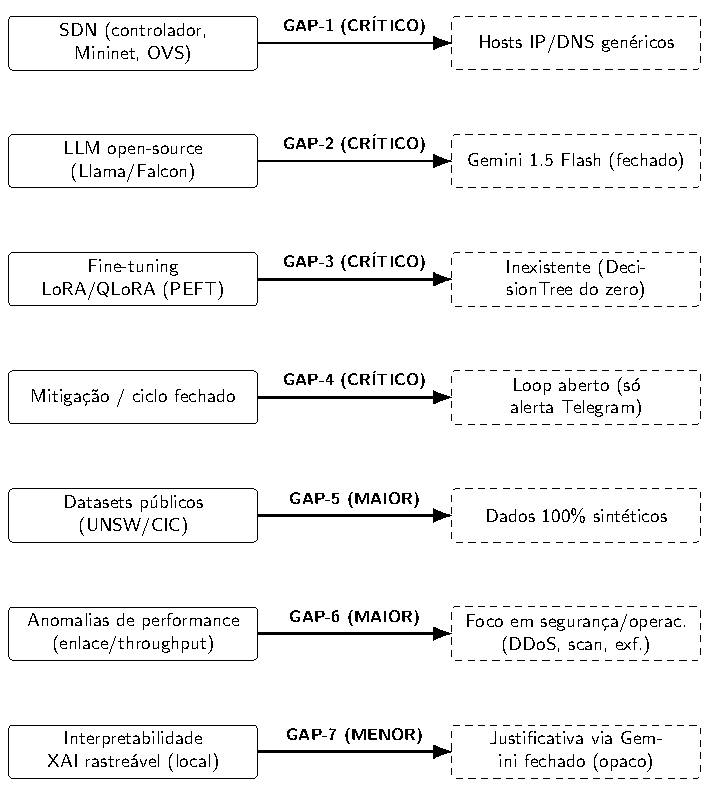
\includegraphics[width=0.82\textwidth]{fig_gaps}
  \caption{Taxonomia de gaps estruturais entre o projeto norteador e o NOC
  Lite. Fonte: elaborada por Chris.}
  \label{fig:gaps}
\end{figure}

O GAP-1 caracteriza a ausência de SDN: o projeto fundamenta toda a proposta
no paradigma SDN, enquanto o NOC Lite monitora hosts IP/DNS arbitrários, sem
controlador, topologia virtualizada ou planos separados \cite{rA19}. O GAP-2
diz respeito ao modelo fechado: o projeto exige LLMs \textit{open source} e
classifica explicitamente o Gemini como modelo fechado \cite{rRODRIGUES}; o
sistema, porém, o utiliza em regime zero-shot \cite{rA317}. O GAP-3 revela a
ausência de LoRA/QLoRA: a seção de PEFT do projeto não tem correspondente, e
o único modelo treinável é uma árvore de decisão do zero \cite{rA41,rA42}. O
GAP-4 aponta o loop aberto: a classificação por IA não está integrada ao laço
de detecção, de modo que o ciclo observa e alerta, sem atuação autônoma
\cite{rA133}. O GAP-5 remete aos dados sintéticos: o treino e o few-shot
repousam no simulador, ausente a validação cruzada com UNSW-NB15
\cite{rA512}. O GAP-6 diz respeito ao escopo: o foco do projeto é
performance (congestionamento, falha de enlace, degradação de desempenho),
ao passo que o sistema privilegia classes de segurança \cite{rA512}. Por fim,
o GAP-7 associa a interpretabilidade a modelo fechado: a justificativa provém
de modelo opaco, fragilizando a promessa de XAI do projeto \cite{rA511,rA52}.

% =====================================================================
\section{Discussão}
\label{sec:discussao}

\subsection{Convergências preservadas}
\label{sec:convergencias}

Apesar dos desalinhamentos estruturais, o NOC Lite honra parcela da intenção
do projeto em pontos que não devem ser subestimados. O primeiro ponto é a
presença de baselines de comparação: o sistema implementa exatamente a
heurística e a árvore de decisão exigidas, permitindo comparação direta lado
a lado \cite{rA210,rA217}, o que materializa o objetivo específico de avaliar
o desempenho da abordagem generativa contra referências clássicas. O segundo
ponto é a tokenização de métricas: \texttt{tokenise\_metrics} converte o
vetor numérico em representação semiestruturada, alinhada à recomendação de
conversão textual \cite{rA616,rA431}, antecipando a ponte de entrada que um
LLM ajustado por LoRA consumiria. O terceiro ponto é a justificativa textual
ou XAI: todos os classificadores retornam \texttt{explanation}, atendendo ao
objetivo qualitativo de interpretabilidade \cite{rA511,rA537}, ainda que com
reserva quanto à rastreabilidade do modelo. O quarto ponto é a medição de
tempo de resposta: o endpoint mede \texttt{latency\_ms} de cada
classificador, entregando a métrica de desempenho exigida \cite{rA31}. O
quinto ponto é a captura de métricas resumidas de rede: SLA, jitter,
tendência e health-score capturam latência, perda e jitter, coincidentes com
as métricas de performance do projeto \cite{rA19}. Esses cinco pontos formam
o alicerce sobre o qual a evolução proposta deve ser construída.

\subsection{Limitações e ameaças à validade}
\label{sec:ameacas}

A limitação mais severa é o viés de dados sintéticos: o classificador de ML é
treinado 100\% com o próprio simulador, que compartilha os mesmos limiares da
heurística; a árvore aprende essencialmente a copiar a heurística em forma de
árvore, com alto desempenho no sintético e provável colapso em produção
\cite{rA414,rA615}. A confiança não é calibrada: a do Gemini é
autorreportada e a do ML é probabilidade de folha não calibrada
\cite{rA532}, tornando a comparação entre classificadores metodologicamente
assimétrica. A orquestração está ausente, pois a classificação encontra-se
fora do ciclo de monitoramento, impossibilitando detecção contínua. Na
validade externa, a ausência de datasets públicos impede a comparação com o
estado da arte \cite{rA65,rA630}.

As ameaças à validade interna incluem a dependência de API externa paga
(Gemini) e a fragilidade do parser JSON, que checa apenas a presença da chave
\texttt{classification}. As ameaças à validade de construção dizem respeito
aos limiares fixos de 50~Mb/s e 120~ms, universais e sem baseline por
host/link, gerando falsos positivos em enlaces de capacidades distintas
\cite{rA21}. Tais fragilidades não invalidam o sistema como protótipo de
diagnóstico, mas restringem sua pretensão de cumprir a proposta norteadora em
sua plenitude.

% =====================================================================
\section{Diretrizes de Arquitetura para Alinhamento}
\label{sec:diretrizes}

Para reduzir a distância entre o NOC Lite e o projeto, propõe-se uma evolução
arquitetural incremental, respeitando o que já existe e fechando os sete gaps.
O ponto central é a transição de um loop aberto para um ciclo fechado com LLM
\textit{open source}, LoRA e mitigação, conforme a Figura~\ref{fig:ciclo}. A
sequência de evolução, espelhando o cronograma do projeto, desdobra-se nos
seguintes passos. O primeiro passo é a substituição do modelo fechado por um
LLM local (fecha GAP-2 e GAP-3): introduzir um contêiner de inferência local
(vLLM/llama.cpp/Ollama) servindo Llama 3 (7--13B) ou Falcon via endpoint
compatível com OpenAI, substituir \texttt{gemini-1.5-flash} por cliente HTTP
local e aplicar LoRA/QLoRA (rank 16--32, alpha 32) sobre o modelo base,
reutilizando os prompts de \texttt{tokenise\_metrics} \cite{rA41,rA42,rA312}.
O segundo passo é a criação de um pipeline de dados com datasets públicos
(fecha GAP-5): módulo \texttt{data\_ingest} que baixa e normaliza UNSW-NB15,
CSE-CIC-IDS2018 e Synthetic SDN para o schema de features, treinando LoRA e a
árvore com dados reais, preservando o simulador para demonstração
\cite{rA61,rA64}. O terceiro passo é o ambiente SDN e o fechamento do ciclo
(fecha GAP-1 e GAP-4): contêiner Mininet + controlador Ryu que emule a
topologia e exponha telemetria de enlace/fluxo; generalização de
\texttt{Host}/\texttt{CheckResult} para telemetria de fluxo SDN; criação de
\texttt{mitigation\_engine} que mapeia \texttt{classification} em ação
corretiva (re-rota, QoS, drop de fluxo) via NorthBound API do controlador;
integração do classificador dentro do \texttt{MonitorEngine}, fechando o
ciclo \cite{rA14,rA116,rA133}. O quarto passo é o realinhamento do catálogo
de anomalias (fecha GAP-6): separar claramente performance SDN
(congelamento de enlace, falha de enlace, degradação de throughput/jitter) de
segurança/operacional (DDoS, port scan, exfiltração, host down), priorizando
a primeira família \cite{rA512}. O quinto passo é a preservação dos pontos
fortes: manter \texttt{tokenise\_metrics}, o par baseline heurístico + ML, a
medição de \texttt{latency\_ms} e o formato de \texttt{explanation} como base
do novo pipeline \cite{rA616,rA431}. O sexto e último passo é o roadmap de
alinhamento experimental: contêiner de LLM \textit{open source} local +
\texttt{tokenise\_metrics} em zero-shot; ingestão dos três datasets + treino
LoRA/QLoRA; Mininet + controlador + telemetria de fluxo;
\texttt{mitigation\_engine} + integração da classificação no
\texttt{MonitorEngine}; e fechamento do ciclo com avaliação comparativa
(heurística vs. ML vs. LLM \textit{open source} com/sem LoRA), reutilizando
\texttt{latency\_ms} e acrescentando acurácia e consistência.

\begin{figure}[H]
  \centering
  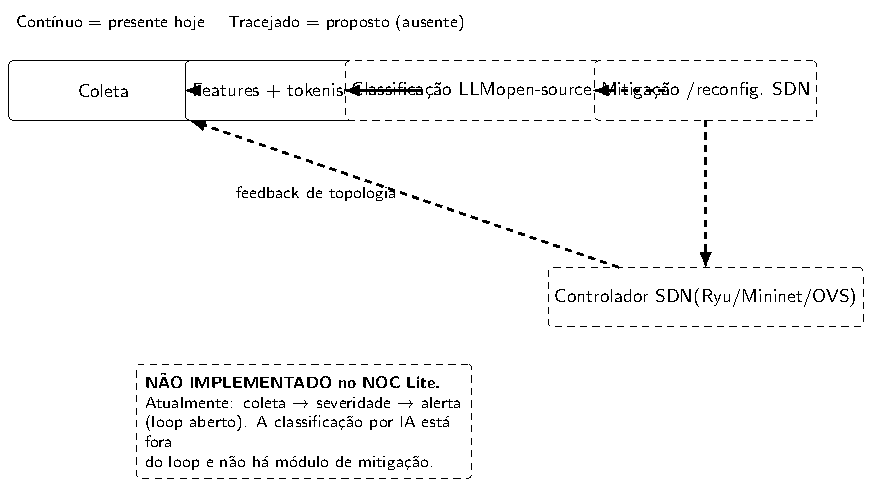
\includegraphics[width=0.85\textwidth]{fig_ciclo_fechado_proposto}
  \caption{Arquitetura proposta de ciclo fechado: coleta (SDN + hosts)
  $\rightarrow$ tokenização $\rightarrow$ classificação (LLM \textit{open
  source} + LoRA) $\rightarrow$ mitigação (módulo de ação) $\rightarrow$
  reconfiguração via controlador. Fonte: elaborada por Chris.}
  \label{fig:ciclo}
\end{figure}

% =====================================================================
\section{Conclusão}
\label{sec:conclusao}

O presente trabalho correlacionou o projeto de pesquisa que propõe detecção e
mitigação de anomalias em SDN com LLMs \textit{open source} ajustados por
PEFT/LoRA \cite{rRODRIGUES} com o sistema efetivamente implementado, o NOC
Lite. Evidenciou-se que o sistema realiza com sucesso a parcela de baselines e
de representação textual do projeto -- heurística, árvore de decisão,
tokenização de métricas, justificativa textual e medição de latência -- mas
diverge estruturalmente nos eixos centrais da proposta. Especificamente, o
NOC Lite monitora hosts genéricos e não SDN; emprega o modelo fechado Gemini
em vez de LLM \textit{open source}; não aplica LoRA/QLoRA; não realiza
mitigação nem opera em ciclo fechado; e depende exclusivamente de dados
sintéticos, sem validação cruzada com datasets públicos.

Tais gaps não são ajustes pontuais: exigem evolução arquitetural substantiva,
sintetizada nas diretrizes de um ciclo fechado com LLM local, LoRA e módulo
de mitigação. As convergências identificadas funcionam como alicerce seguro
sobre o qual construir essa evolução, uma vez que o
\texttt{tokenise\_metrics}, os baselines e a medição de latência já cumprem
objetivos específicos do projeto. Como trabalho futuro, recomenda-se a
implementação do \texttt{mitigation\_engine} e a condução do experimento
comparativo head-to-head entre LLM \textit{open source} ajustado por QLoRA e
LLM fechado zero-shot sobre o mesmo conjunto de métricas de rede -- lacuna
exatamente apontada pela literatura \cite{rA49,rA630}. A realização desse
experimento é o passo necessário para que a implementação deixe de ser um
diagnóstico por similaridade e passe a constituir, de fato, a validação
empírica da proposta norteadora.

% =====================================================================
\bibliography{referencias_autor_data}

\end{document}
